\documentclass[lualatex,ja=standard]{bxjsarticle}

\setpagelayout{noheadfoot,top=1cm,bottom=1cm,left=2cm,right=2cm}
\setlength{\footskip}{6mm}

% タイトル情報(必要に応じて編集)
\title{実験レポートタイトル}
\author{作成者名}
\date{\today}

% パッケージ類
\usepackage{graphicx}   % 画像を挿入するため
\usepackage{amsmath}    % 数式を使うため
\usepackage{amssymb}    % 数式を使うため
\usepackage{caption}    % 図表のキャプション
\usepackage{subcaption} % サブキャプション
\usepackage{siunitx}    % 数式の設定
\usepackage{booktabs}   % 表のスタイル
\usepackage{multirow}   % 表のスタイル
\usepackage{pdfpages}   % 表紙の挿入
\usepackage{enumitem}   % 箇条書き
\usepackage{titlesec}   % セクションのスタイル
\usepackage{luatexja-fontspec} % フォント設定
\usepackage{hyperref}   % 図表へのリンク
\usepackage{xspace}     % スタイルの装飾
\usepackage{makecell}   % 表のセルを結合するため
\usepackage{ascmac}     % 図の枠を作成するため
\usepackage{listings}   % ソースコードの表示

% フォント
\setmainjfont{IPAexMincho} 
\AtBeginDocument{%
  \fontsize{10.5pt}{16pt}\selectfont
}

% 樹形図
\usepackage{tikz}
\usetikzlibrary{graphs, graphdrawing, arrows.meta, calc}
\usegdlibrary{trees}  % trees 用ライブラリ

% セクションスタイル
\newcommand{\mysectionstyle}[2]{%
  \sffamily         % 欧文・数字→サンセリフ
  \gtfamily         % 日本語→ゴシック
  \bfseries
  \fontsize{#1}{#2}\selectfont
}

% セクションのスタイル
\titleformat{\section}
  {\mysectionstyle{12pt}{16pt}}
  {\mysectionstyle{12pt}{16pt}\thesection.}
  {0.7em}{}
\titlespacing*{\section}{0em}{1em}{0em}

% サブセクションのスタイル
\titleformat{\subsection}
  {\mysectionstyle{10.5pt}{16pt}}
  {\mysectionstyle{10.5pt}{16pt}\thesubsection.}
  {0.7em}{}
\titlespacing*{\subsection}{0em}{0.5em}{0em}

% サブサブセクションのスタイル
\titleformat{\subsubsection}
  {\mysectionstyle{10.5pt}{12pt}}
  {\mysectionstyle{10.5pt}{12pt}\thesubsubsection.}
  {0em}{}
\titlespacing*{\subsubsection}{0em}{0.5em}{0em}

% パラグラフのスタイル
\titleformat{\paragraph}
  {\mysectionstyle{10.5pt}{12pt}}
  {\mysectionstyle{10.5pt}{12pt}\theparagraph.} 
  {0em}{}
\titlespacing*{\paragraph}{0em}{0em}{0em}

% サブパラグラフのスタイル
\titleformat{\subparagraph}
  {\mysectionstyle{8pt}{12pt}}
  {\mysectionstyle{8pt}{12pt}\thesubparagraph.}
  {0em}{}
\titlespacing*{\subparagraph}{0em}{0em}{0em}

% 和文キャプション
\renewcommand{\figurename}{図}
\renewcommand{\tablename}{表}
\renewcommand{\refname}{参考文献}
\renewcommand{\lstlistingname}{ソースコード}

% autoref の和文化
\renewcommand*{\figureautorefname}{図}
\renewcommand*{\tableautorefname}{表}
\renewcommand*{\equationautorefname}{式}
\renewcommand*{\subfigureautorefname}{図}

\captionsetup[subfigure]{labelformat=simple}
\renewcommand*{\thesubfigure}{(\alph{subfigure})}

\captionsetup[subtable]{labelformat=simple}
\renewcommand*{\thesubtable}{(\alph{subtable})}

% 単位の設定
\sisetup{
  detect-all,
  per-mode = symbol,
  range-phrase = --,
}
\NewDocumentCommand{\sibr}{m}{\,\text{[\si{#1}]}} 

% ソースコード用の設定
\lstset{
  basicstyle={\ttfamily},
  identifierstyle={\small},
  commentstyle={\small\itshape},
  keywordstyle={\small\bfseries},
  ndkeywordstyle={\small},
  stringstyle={\small\ttfamily},
  frame={tb},
  breaklines=true,
  columns=[l]{fullflexible},
  numbers=left,
  xrightmargin=0em,
  xleftmargin=3em,
  numbersep=1em,
  numberstyle={\scriptsize},
  stepnumber=1,
  lineskip=-0.5ex
}

% リンクの色設定
\hypersetup{
  colorlinks=true,
  linkcolor=black,
  citecolor=black,
  urlcolor=black
}

% 参考文献の設定
\usepackage[backend=biber,style=numeric,sorting=none]{biblatex}
\addbibresource{refs.bib}

% 参考文献の書式設定
\DeclareDelimFormat{multinamedelim}{,}
\DeclareDelimFormat{finalnamedelim}{,}
\DeclareDelimFormat{nameyeardelim}{,}
\DeclareFieldFormat{title}{#1}
\DeclareFieldFormat{journaltitle}{#1}
\renewcommand*{\newunitpunct}{,}
\DeclareCiteCommand{\cite}
  {\usebibmacro{prenote}}
  {\mkbibsuperscript{[\printfield{labelnumber}]}}
  {\multicitedelim}
  {\usebibmacro{postnote}}

% 書籍フォーマット
\DeclareBibliographyDriver{book}{%
  \printnames{author}:%
  \printfield{title},%
  \printfield{pages},%
  \printlist{publisher} (\printfield{year})%
  \finentry
}

% 雑誌論文フォーマット
\DeclareBibliographyDriver{article}{%
  \printnames{author}:%
  \printfield{title},%
  \printfield{journaltitle},%
  Vol.\printfield{volume},%
  \printfield{pages}(\printfield{year})%
  \finentry
}

% 段落設定
\setlength{\parskip}{0.5em}
\setlength{\parindent}{1em}
\makeatletter
\AtBeginDocument{
  \let\@afterindentfalse\@afterindenttrue
}
\makeatother

\begin{document}

% 表紙(wordから出力した表紙をcover/CN.pdfに保存)
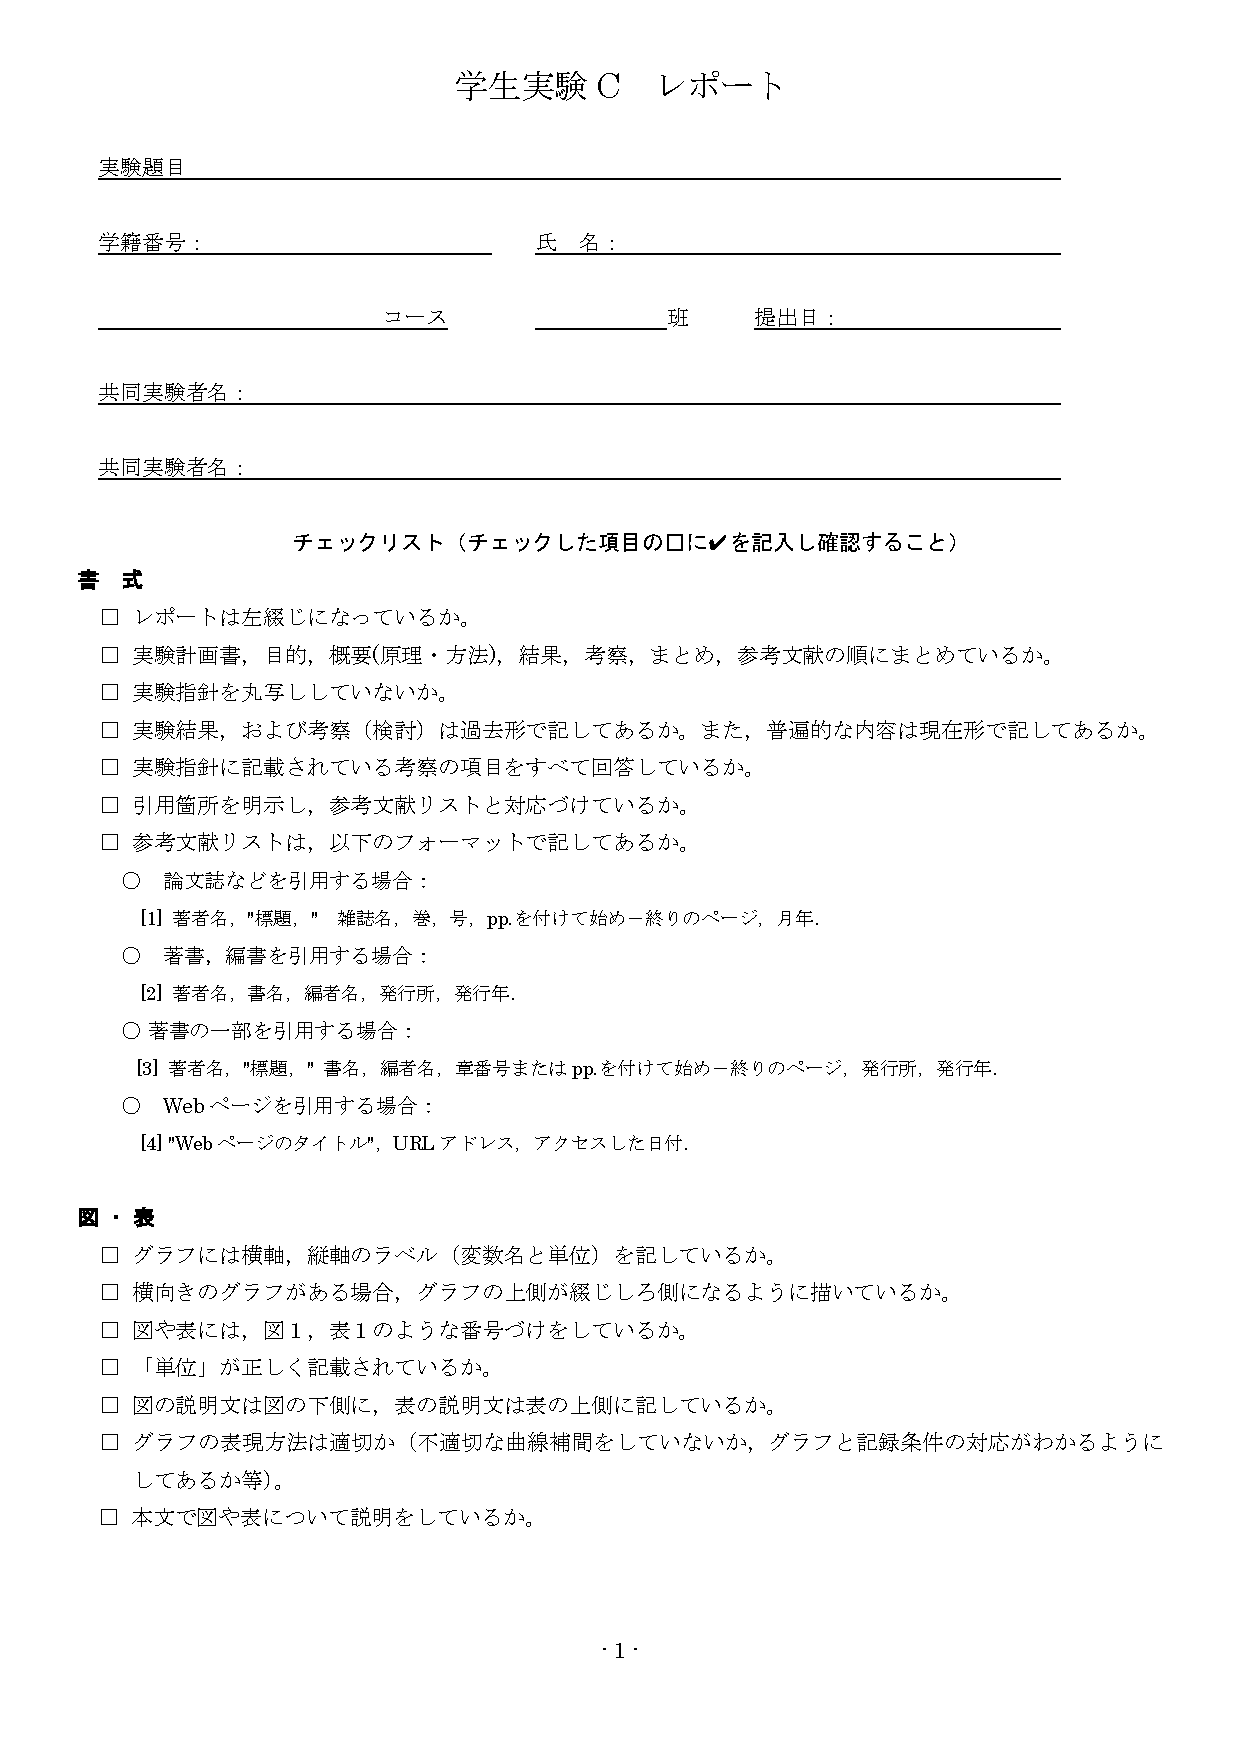
\includepdf[pages=1]{cover/CN.pdf}

\section{実験の目的}
本実験の目的をここに記述する.

\section{原理}
実験の理論的背景を簡潔に記述する.樹形図は\autoref{fig:tree-diagram}のように作成する.ChatGPTを使用して作成すると良い.

\begin{figure}[htbp]
  \centering
  % 必要に応じてTikZ図を編集または削除
  \begin{tikzpicture}[font=\normalsize, node distance=3cm and 2cm, every node/.style={draw=none, anchor=west}, >={Latex}]
    \node (root) at (0,0) {現象A};
    \node (child1) at ($(root)+(4,0.5)$) {要因1};
    \node (child2) at ($(root)+(4,-0.5)$) {要因2};
    \draw[->] (root.east) -- (child1.west);
    \draw[->] (root.east) -- (child2.west);
  \end{tikzpicture}
  \caption{現象の分類例}
  \label{fig:tree-diagram}
\end{figure}

\section{実験の方法}

\subsection*{[使用器具]}

\begin{itemize}
  \item 使用器具1
\end{itemize}

\subsection{実験概要}
ここに全体の手順や測定方法の概要を記述する.

\subsection{個別手順}
\subsubsection*{[手順例]}
\begin{enumerate}
  \item 装置の初期設定
  \item 測定値の取得
  \item 注意点や補足説明(\textbf{安全注意}など)
\end{enumerate}

\section{実験結果}

\begin{table}[htbp]
  \centering
  \caption{測定結果の例}
  \label{tab:example}
  \begin{tabular}{cccc}
    \toprule
    条件1 & 条件2 & 条件3 & 条件4 \\
    \midrule
    値1 & 値2 & 値3 & 値4 \\
    \bottomrule
  \end{tabular}
\end{table}

\begin{equation}
  y = a x + b \sibr{\meter\per\second}
  \label{eq:line}
\end{equation}
\autoref{eq:line}は測定結果の線形関係を表す.

作成したプログラムも\autoref{lst:python-example}のように表示可能.

\begin{lstlisting}[language=Python, caption=Pythonの例, label=lst:python-example]
  print("Hello, World!")

  def add(a, b):
      return a + b
  result = add(1, 2)
  print("Result:", result)
\end{lstlisting}

画像の挿入例は\autoref{fig:example}の通り.

\begin{figure}[htbp]
  \centering
  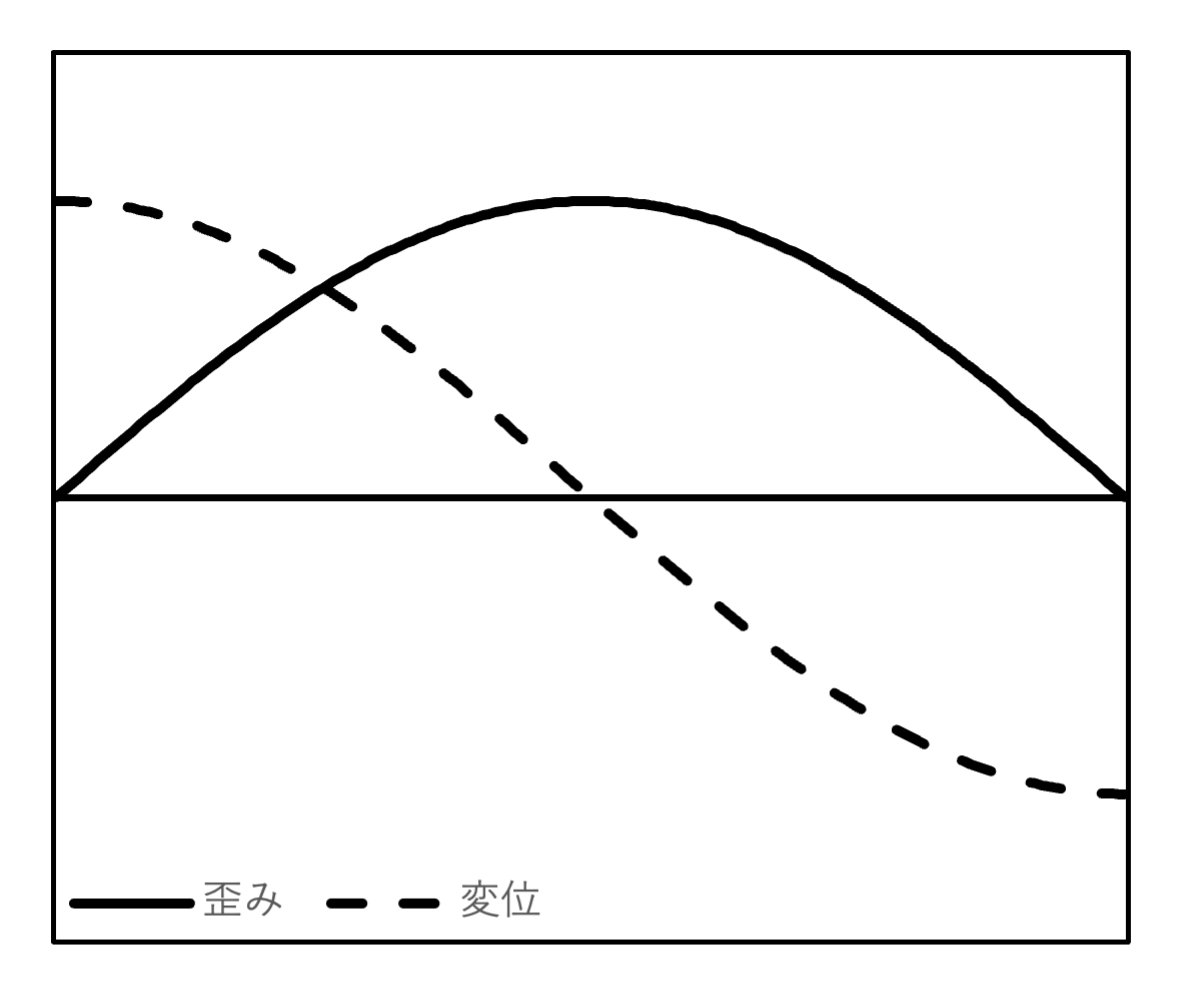
\includegraphics[width=0.5\textwidth]{img/CN/graph.png}
  \caption{画像の例}
  \label{fig:example}
\end{figure}

\section{考察}
実験結果に基づいて考察を記述する.たとえば,傾向の説明,理論との一致・不一致,実験誤差の要因などを検討する.

このように参考文献の明示もできる\cite{nist811-si-guide}.

\section{結論}
実験全体の要点を簡潔にまとめる.たとえば,
\begin{itemize}
  \item 結果から得られる一般的な知見
  \item 今後の課題や応用可能性
\end{itemize}

\printbibliography[title=<参考文献>]

\end{document}
